\documentclass[../main.tex]{subfiles}

\begin{document}
In questo capitolo si descrive la progettazione e lo sviluppo di una riproduzione del famoso gioco Snake adottando il paradigma Functional Reactive Programming. Al requisito non funzionale dell'utilizzo del paradigma FRP e del linguaggio di programmazione Scala si aggiunge anche quello dell'utilizzo della libreria \textit{Sodium}, analizzata nel capitolo precedente e scelta per la chiarezza e la completezza (ovvero il rispetto del paradigma FRP) delle API fornite.

I requisiti funzionali della applicazione \textit{FRP Snake} sono:
\begin{itemize}
    \item Il serpente si muove di una posizione nelle direzioni su, giu, destra e sinistra ed ha una dimensione iniziale pari a 1.
    \item Il numero di elementi che il serpente può mangiare è costante durante tutta la durata del gioco: quando il serpente mangia un elemento deve essere aggiunto un nuovo elemento.
    \item Gli elementi che il serpente può mangiare sono di due tipi: "buono", aumenta il punteggio complessivo di 100 punti e "cattivo", diminuisce il punteggio complessivo di 100 punti. In entrambi i casi il serpente aumenta la sua dimensione di 1 unità.
    \item La velocità di movimento del serpente è settata a 1 unità al secondo e può essere modificata a runtime in qualunque momento.
    \item Una partita si conclude quando il serpente è annodato.
\end{itemize}

\section{Progettazione}

\subsection{Input e Output}
Il seguente diagramma rappresenta gli input e gli output dell'applicazione in relazione agli elementi della GUI:
\begin{description}
  \item[directionInput] - Gli eventi associati alla pressione dei tasti "freccia su" (\textit{VK\_UP}), "freccia giu" (\textit{VK\_DOWN}), "freccia destra" (\textit{VK\_RIGHT}) e "freccia sinistra" (\textit{VK\_LEFT}) modificano il valore dell'input \textit{directionInput}, utilizzato per computare il movimento del serpente.
  \item[statusInput] - Gli eventi associati alla pressione dei tasti "S" (\textit{VK\_S}), "Q" (\textit{VK\_Q}) e "P" (\textit{VK\_P}) modificano il valore dell'input \textit{statusInput}, utilizzato rispettivamente per avviare/riprendere, terminare o sospendere la partita in corso.
  \item[speedInput] - Gli eventi associati alla pressione dei tasti "U" (\textit{VK\_U}) e "D" (\textit{VK\_D}) modificano il valore dell'input \textit{speedInput}, utilizzato per computare la velocità di movimento del serpente (frequenza dell'engine di gioco).
  \item[snakeOutput] - Stream attivato ogni volta che viene modificato il corpo del serpente, in seguito al movimento o all'eliminazione di un elemento "cibo".
  \item[foodOutput] - Stream attivato ogni volta che viene modificato l'insieme degli elementi "cibo" presenti nel mondo di gioco.
  \item[scoreOutput] - Stream attivato ogni volta che viene modificato il punteggio, ovvero quando viene eliminato un elemento "cibo" e quindi aumentata la dimensione del corpo del serpente.
\end{description}

\begin{figure}[H]
\centering
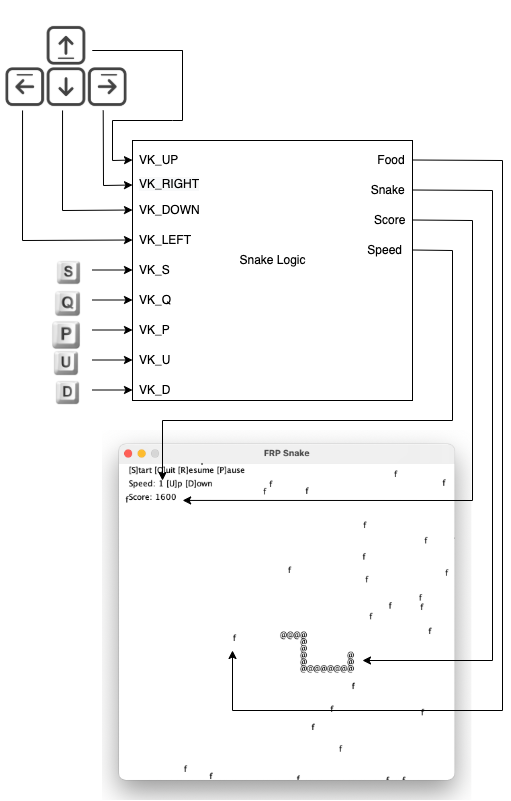
\includegraphics[width=0.9\textwidth]{img/frp-scala-Page-2.drawio.png}
\caption{Input/Output del programma FRP in relazione alla GUI}
\end{figure}

Data la definizione degli input e degli output della applicazione, la seguente figura rappresenta il diagramma delle dipendenze, ovvero la logica in termini FRP che permette la computazione degli output in reazione alla modifica dei valori in input:
\begin{figure}[H]
\centering
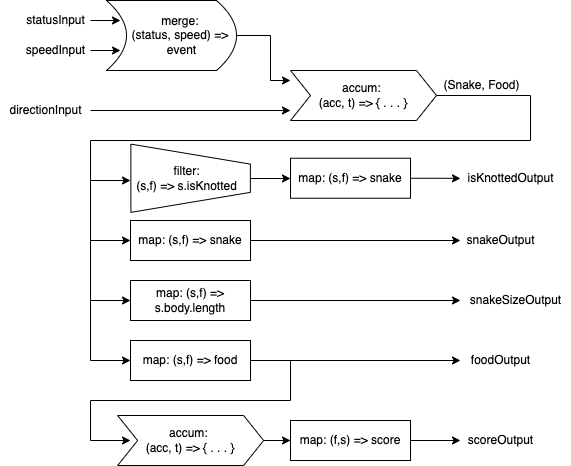
\includegraphics[width=0.9\textwidth]{img/frp-scala-Page-5.drawio.png}
\caption{Grafo delle dipendenze: FRP Snake}
\end{figure}
\end{document}

\section{Implementazione}
Il mondo di gioco 2D è modellato come un insieme di punti cardinali (\textit{Position}) e un confine dato dai limiti inferiori e superiori nei due assi x,y (\textit{Boundary}). Sfruttando le \textit{type-classes} fornite da Scala, i due concetti assumono rispettivamente il significato di \textit{Tupla2} (x,y) e \textit{Tupla4} (xMin, xMax, yMin, yMax).
\begin{lstlisting}[language=Javascript, caption=Definizione dei concetti rappresentanti il mondo 2D di gioco tramite \textit{type-classes}.]
object World {
  type Position = (Int,Int)
  type Boundary = (Int,Int,Int,Int)
}
\end{lstlisting}

L'engine FRP della applicazione, ossia la logica che valuta le dipendenze mappando gli input con gli output, è dato da due componenti principali:
\begin{description}
  \item[Engine] - Si occupa dell'avanzamento/terminazione del gioco e della velocità di gioco. Lo stream di output di questo componente si attiva con una certo periodo (in millisecondi: \textit{1000 / speedInput.sample}) pilotando la computazione della nuova posizione del serpente. dedicato.
  \begin{figure}[H]
\centering
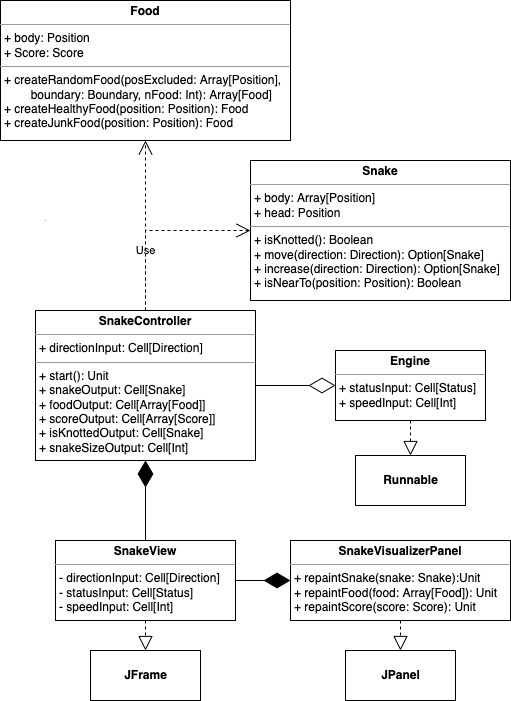
\includegraphics[width=0.9\textwidth]{img/frp-scala-Page-6.drawio.png}
\caption{Diagramma delle classi - FRP Snake}
\end{figure}
  \item[SnakeController] - Implementa in termini FRP il core del gioco Snake. I diversi stream di output di questo componente permettono alla parte grafica di aggiornare la GUI in reazione alla attivazione. All'avvio (\textit{start}) del componente viene inizializzato il mondo di gioco, ovvero serpente e cibo, e viene sottomesso il componente \textit{Engine} ad un apposito \textit{ExecutorService}.
\end{description}


\begin{lstlisting}[language=Javascript, caption=Generazione random delle entità "Food" tramite for-comprehension.]
def createRandomFoods(positionToBeExcluded: Array[Position], boundary: Boundary, nFood: Int): Array[Food] = {
    (for {
      i <- 0 until nFood
      position = (Random.between((boundary._1/10).round*10, (boundary._2/10).round*10), Random.between((boundary._3/10).round*10, (boundary._4/10)*10))
      if !positionToBeExcluded.contains(position)
    } yield if((position._1 + position._2) % 2 == 0) Food.createHealthyFood(position) else Food.createJunkFood(position)).toArray
  }
\end{lstlisting}

\begin{lstlisting}[language=Javascript, caption=Pimp my Library pattern - Aggiunta feature all'entità \textit{Snake} per vincolare il movimento all'interno del "mondo" di gioco.]
implicit class BoundedSnake(snake: Snake) {
    def bound(boundary: Boundary): Snake = {
      Snake(snake.body.map(pos => {
        var tmpPos = pos
        if (pos._1 > boundary._2) tmpPos = (boundary._1 + 10, tmpPos._2)
        else if (pos._1 <= boundary._1) tmpPos = (boundary._2 - 10, tmpPos._2)
        else tmpPos = (pos._1, tmpPos._2)
    
        if (pos._2 > boundary._4) tmpPos = (tmpPos._1, boundary._3 + 10)
        else if (pos._2 <= boundary._3) tmpPos = (tmpPos._1, boundary._4 - 10)
        else tmpPos = (tmpPos._1, pos._2)
    
        logger.debug(s"pre: ${pos} - post: ${tmpPos}")
        tmpPos
      }))
    }
}
\end{lstlisting}
